\section{Durchführung}
\label{sec:Durchführung}

In \autoref{fig:1} befindet sich der Aufbau des Versuchs.
\begin{figure}[H]
    \centering
        \centering
        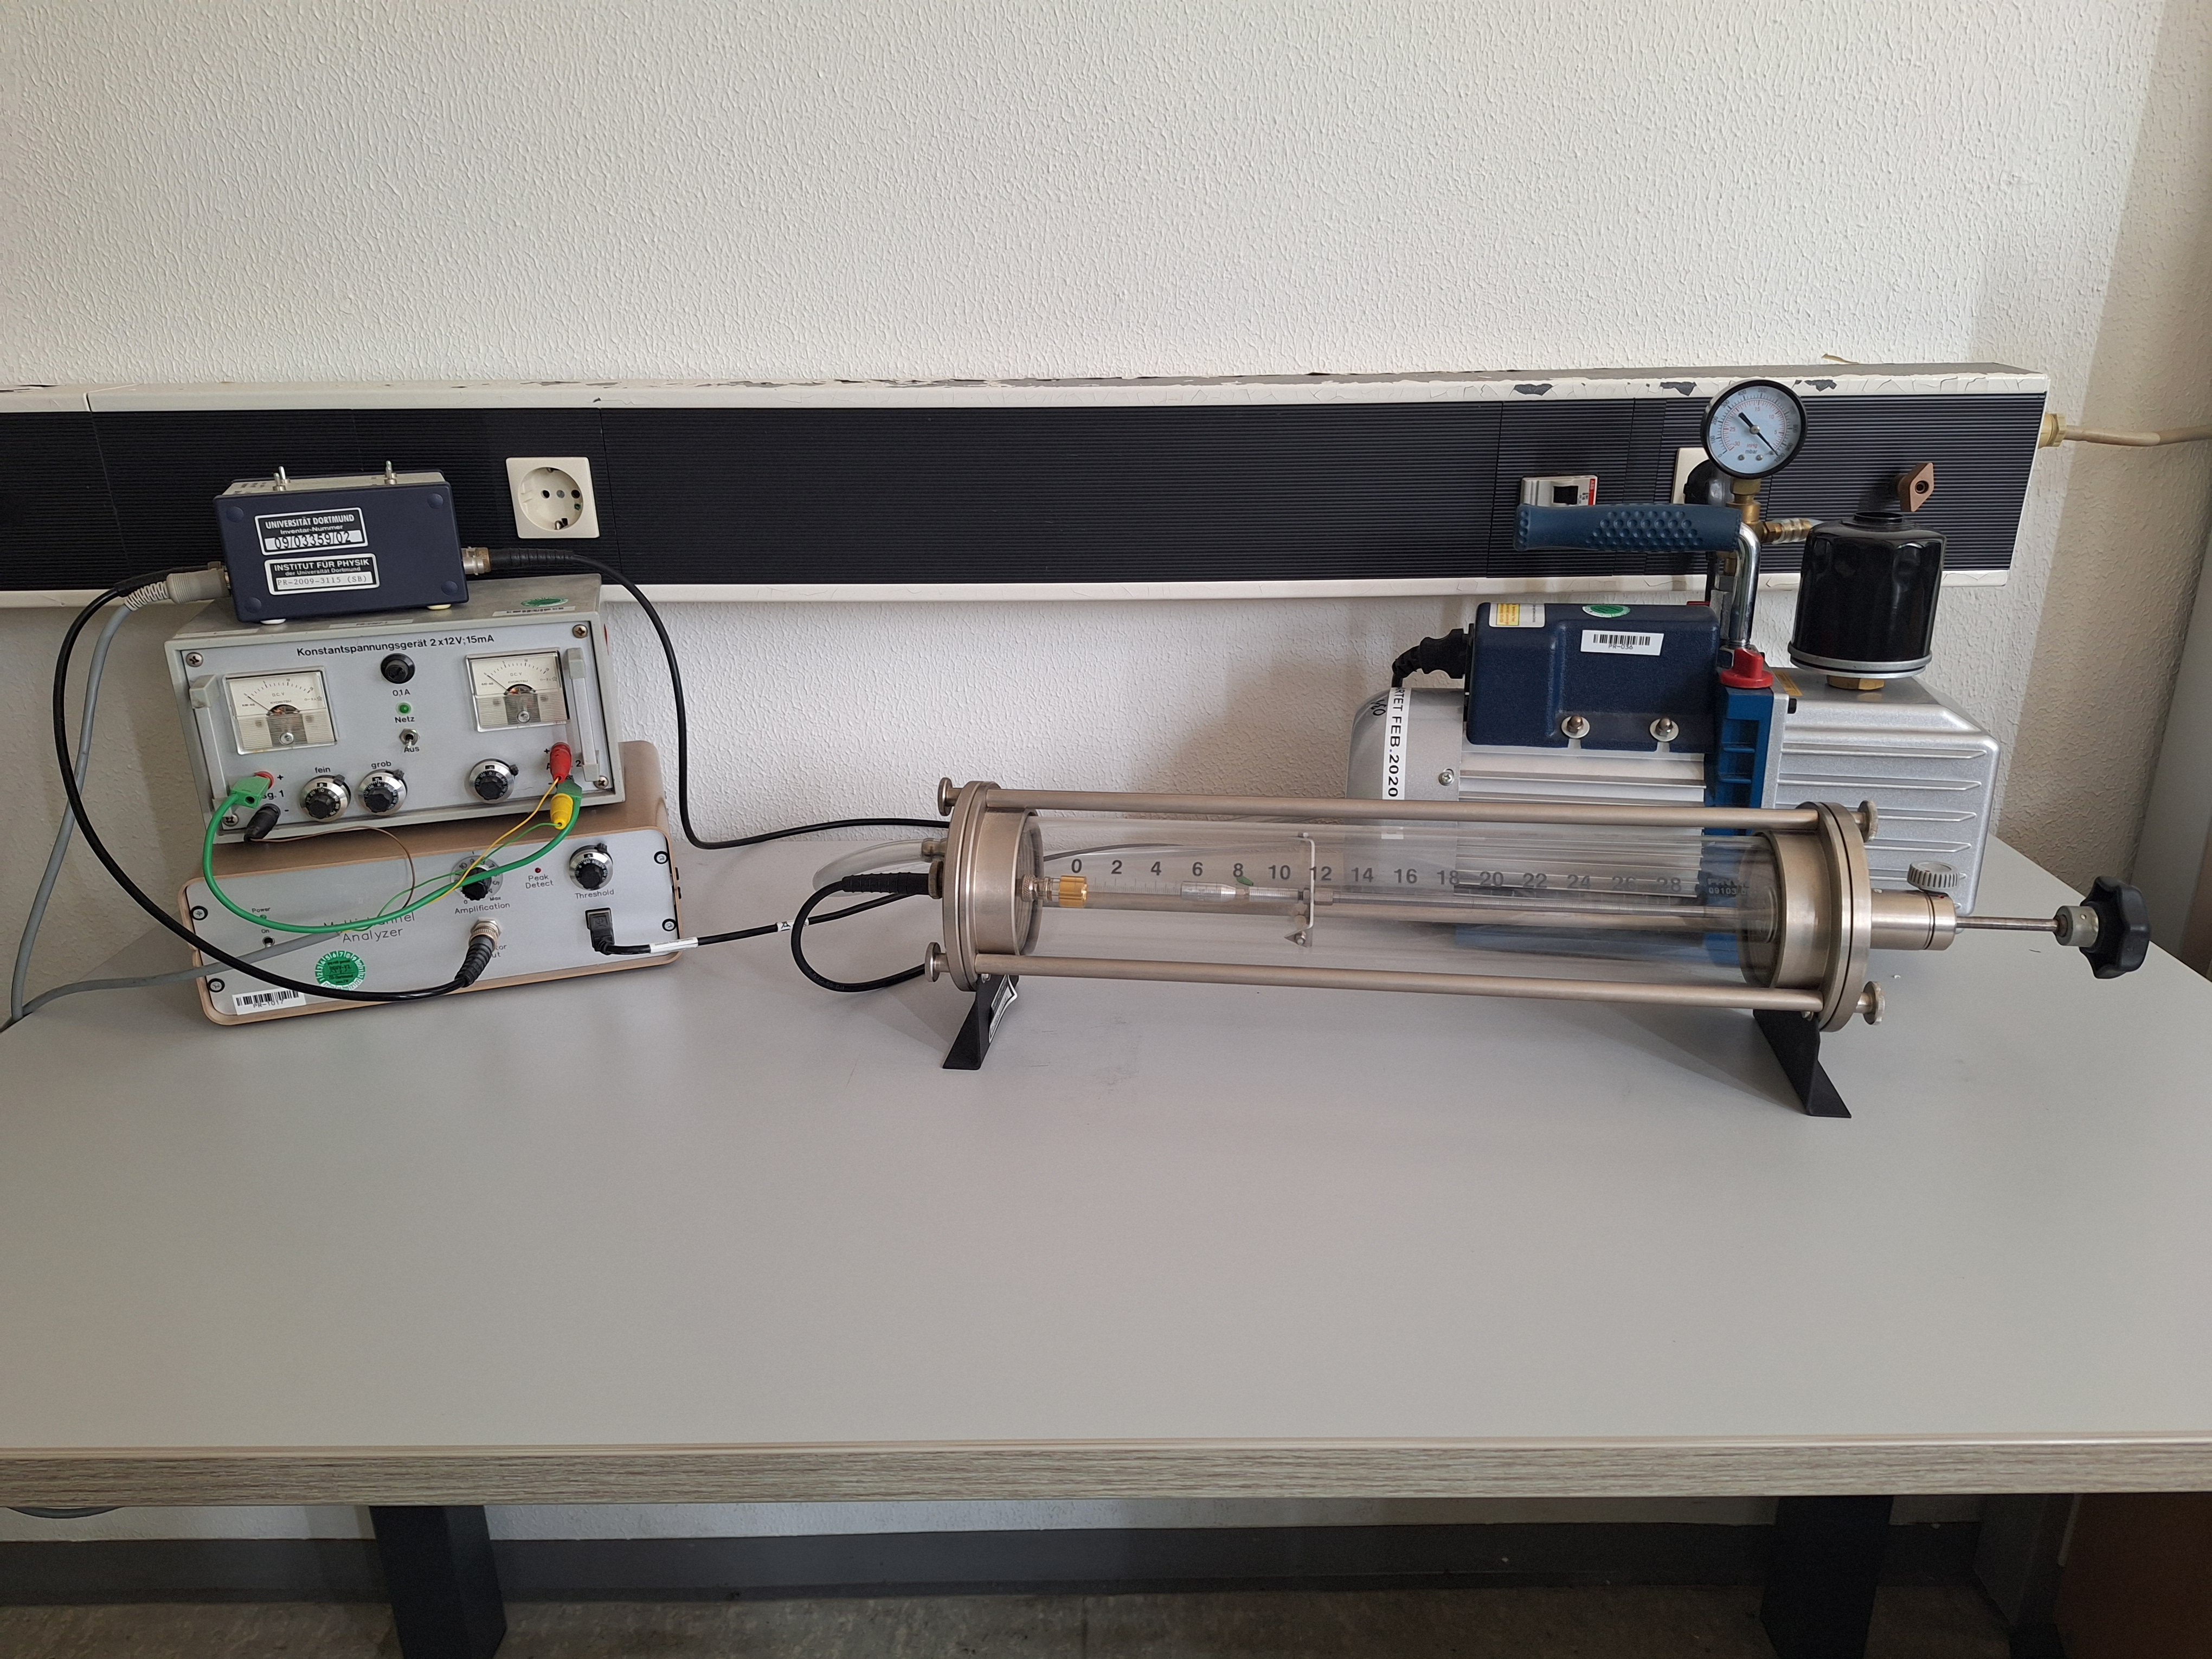
\includegraphics[width=\textwidth]{bilder/versuch.jpg}
        \caption{Aufbau des Versuchs.}
    \hfill
    \label{fig:1}
\end{figure}
\noindent Zu sehen ist der Glaszylinder mit Skala in der Mitte, dieser beinhaltet 
das $\alpha$-Präparat und den Halbleiter-Detektor, dessen Distanz $x_0$ variiert 
werden kann. Als Quelle für die Strahlung wird Amercium mit einer Halbwertszeit 
von $T_{1/2} = \SI{458}{a}$. Der Detektor ist ein Halbleiter-Sperrschichtzähler, 
dieser detektiert Strahlung, indem er Elektronen-Loch-Paare als messbaren 
Stromimpuls wahrnimmt, nachdem diese von geladenen Teilchen produziert wurden. 
Auf der linken Seite befindet sich die Spannungsversorgung, während sich rechts 
die Vakuumpumpe befindet, um die Röhre zu evakuieren. Jenes geschieht über 
die Reglung mittels eines Schalters hinter der Messuhr. Zusätzlich steht auch 
ein Computer zur Verfügung, welcher die Aufnahme der Daten (pulses und Channels)
mithilfe des Programms \glqq Multichannal Analyzer\grqq \, ermöglicht.
\vspace{0.5em}
\\
\noindent Als erstes wird die Detektionsschwelle des Halbleiter-Sperrschichtzählers 
so eingestellt, dass die Pulse gerade noch detektiert werden (bei Atmosphärendruck). 
Anschließend wird der Zylinder evakuiert und 
die Messung kann beginnen. Bei einem konstanten Druck von erst $0 \unit{\milli\bar}$
kann die Messung starten; die Laufzeit von $t = 120 \unit{\second}$ wird eingestellt 
und die Impulszahl und die Zählrate werden in Abhängigkeit des Drucks notiert. 
Letzteres wird um $50 \unit{\milli\bar}$ erhöht, bis kaum noch etwas detektiert 
wird.
\vspace{0.5em}
\\
\noindent Für die Überprüfung der Statistik des radioaktiven Zerfalls wird 
analog eine Messreihe aufgenommen. Zunächst wird wieder der Zylinder evakuiert, 
dann werden bei $t = 10 \unit{\second}$ die Zerfälle pro Zeit bei $p = 0 \unit{\milli\bar}$
gemessen.